\chapter{Diagnostic et Pronostic des Roulements avec les Réseaux de Neurones}
\label{chapter:diagnostic-and-prognostic-of-bearings-using-neural-networks}
\chapterintrobox{La surveillance des vibrations est vitale pour de nombreux systèmes industriels. Les mesures des vibrations contiennent des informations très utiles sur l'état de santé des équipements et les types de défauts. Néanmoins, obtenir des informations à partir de ces signaux dans des applications réelles se révèle être un processus complexe. Cela est principalement dû à la complexité du problème. Ce chapitre présente plusieurs approches pour le diagnostic et le pronostic des défauts de roulements à l'aide de réseaux de neurones convolutifs.}

\section{Étude de cas: Diagnostique des roulements}%
\label{sec:etude_de_cas_diagnostique_des_roulements}

\begin{wrapfigure}[14]{r}{0.5\textwidth}
    \centering
	\begin{tikzpicture}
	\node (outer) at (3.5,1.2) {\makecell{\small Outer\\Race}};
	\node (inner) at (3.5,0) {\makecell{\small Inner\\Race}};
	\node (ball) at (3.5,-1.2) {\makecell{\small Ball\\(in cage)}};
	
	\node (outer2) at (1.3,1.2) {};
	\node (inner2) at (.3,0) {};
	\node (ball2) at (-.5,-1.2) {};

	\node[inner sep=0] (image) at (0,0) {\includegraphics[width=0.35\textwidth]{figures/skf.jpg}};

	\draw [|->,  thick, red] (outer.west) -- (outer2);
	\draw [|->,  thick, red] (ball) -- (ball2);
	\draw [|->,  thick, red] (inner) -- (inner2);
\end{tikzpicture}
	\caption{Composants d'un roulement}
    \label{figure:skf-bearing-components}    
\end{wrapfigure}

Les données utilisées dans cette section sont des données de vibrations des roulements fournies par Case Western Reserve University (CWRU). Les roulements utilisés dans le test sont des roulements à billes SKF. La figure \ref{figure:skf-bearing-components} montre les différents composants d'un roulement à billes standard. L'essai a été réalisé là où les roulements supportent l'arbre d'un moteur de 2 chevaux dans différentes conditions de charge. 

Les roulements d'essai possèdent des défauts ponctuels qui ont été introduits par électroérosion avec des diamètres de défaut de 0,18 mm, 0,36 mm, 0,53 mm, 0,71 mm et 1,02 mm. Ces défauts ont été introduits dans la bille et les chemins de roulement intérieurs et extérieurs du roulement. Des roulements SKF ont été utilisés pour les défauts de 0,18 mm, 0,36 mm et 0,53 mm, et des roulements équivalents NTN ont été utilisés pour les défauts de 0,71 mm et 1,02 mm. Le tableau \ref{table:cwru-bearings-specification} contient les dimensions des modèles de roulements SKF utilisés et les fréquences correspondantes (en multiples de RPM) associées aux différents types de défauts.

\begin{table}[H]
	\centering
	\begin{tabu}{cc|[1.5pt]cc}
		\tabucline[1.5pt]{-} 
		Dimension		&	Valeur (mm)	&	Défaut 			& Fréquence ($\times$RPM Hz)	\\
		\hline
		Diamètre intérieur	&	25.00		& Chemin intérieur 		& 5.4152\\
		Diamètre extérieur&	52.00		& Chemin extérieur 		& 3.5848 \\
		Épaisseur 		&	15.00		& Cage		& 0.3983 \\
		Diamètre du pas	&	08.03		& Bille	& 4.7135\\
		\tabucline[1.5pt]{-} 
	\end{tabu}
	\caption{Dimensions des roulements CWRU et les fréquences de défauts}
	\label{table:cwru-bearings-specification}
\end{table}

\subsection{Génération de données à partir de vibration}
Les données de vibration non traitées ne peuvent pas être utilisées directement pour entraîner un réseau de neurones. Ce chapitre utilise l'approche proposée dans \cite{Wen2018} pour convertir les données de vibration non traitées en images. La figure \ref{fig:cw_bearings_data_generation} montre le principe de génération de données où les signaux de vibration à une dimension sont convertis en matrices à deux dimensions (images) en transformant des morceaux de longueur 4096 en matrices de 64$\times$64.

\begin{figure}[h]
	\centering
	\includegraphics{figures/cw_bearings_data_generation_fr.pdf}
	\caption{Génération de données par conversion du signal en images 64$\times$64}
	\label{fig:cw_bearings_data_generation}
\end{figure}

Comme mentionné précédemment, plusieurs essais ont été réalisés avec différents types de défauts de roulements (c'est-à-dire des défauts de billes, de chemins de roulement intérieurs et extérieurs) avec différents diamètres de défaut. Les signaux des différents tests sont transformés en images pour servir d'entrée à un réseau de neurones convolutif qui sera entraîné à classer les différents signaux dans les types de défauts correspondants et leurs diamètres. Les signaux sont répartis en 10 classes : trois types de défauts différents et pour chaque type de défaut, il y a trois diamètres de défaut différents, plus un signal de base normal qui appartient au roulement sain. La figure \ref{fig:bearings_faults_samples} montre quelques échantillons des signaux transformés des neuf différents types de défaut/diamètres : 

\begin{figure}[h]
    \centering
	\includegraphics{figures/cw_bearings_faults_samples.pdf}
    \caption{Signaux convertis de différents types de défauts}
    \label{fig:bearings_faults_samples}
\end{figure}

Les signaux des différents types de défauts ont des longueurs variables, ce qui se traduit par un nombre différent d'images synthétisées par type de défaut. Le nombre d'images par type de défaut (classe) est donné par l'équation \ref{equation:labels-per-class} :

\begin{equation}
	N=floor \left(\frac{\text{signal length}}{64\times64}\right)
	\label{equation:labels-per-class}
\end{equation}

Le nombre d'images correspondant à chaque classe est indiqué dans le tableau \ref{table:cw-classes-count}:

\begin{table}[h]
	\centering
	\begin{tabu}{lc}
		\tabucline[1.5pt]{-}
	   Classe 					&	Nombre d'échantillons	\\
	   \hline
	   Normal bearing 			&	295				\\
	   Roller element 0.18mm 	&	146				\\
	   Roller element 0.36mm 	&	116				\\
	   Roller element 0.54mm	&	116				\\
	   Inner race 0.18mm		&	295				\\
	   Inner race 0.36mm		&	116				\\
	   Inner race 0.54mm		&	116				\\
	   Outer race 0.18mm		&	116				\\
	   Outer race 0.36mm		&	116				\\
	   Outer race 0.54mm		&	116				\\
	   \hline
	   Total 					& 1548 				\\
   \tabucline[1.5pt]{-}
   \end{tabu}
   \caption{Nombre d'échantillons pour chaque classe de défauts}
   \label{table:cw-classes-count}
\end{table}
%\end{comment

\subsection{Diagnostic des défauts de roulements à l'aide de réseaux de neurones}
Après avoir généré des données en convertissant des signaux vibratoires bruts en images, ces images servent d'entrée pour un réseau de neurones convolutif.

\subsubsection{Architecture de réseau}
\acrlong{cnn} (\acrshort{cnn}) décrit un type de réseaux de neurones qui convient au traitement des images. Cette section présente l'utilisation de \acrshort{cnn} pour classer les signaux de vibration des roulements qui ont été transformés en images dans les types de défauts correspondants. Les \acrshort{cnn} ont été décrits en détail dans la section \ref{section:cnn}.

Pour effectuer cette tâche de classification, une architecture \acrshort{cnn} est utilisée, le réseau se compose de trois couches convolutionnelles avec des couches MaxPool entre elles, suivies de trois couches Fully-Connected. Tous les détails de cette architecture sont mentionnés dans le tableau\ref{table:bearings-faults-cnn-classifier-architecture}.

\begin{table}[h]
    \centering
    \begin{tabu}{lll}
		\tabucline[1.5pt]{-}
		\textbf{Couche (type)}   & \textbf{Forme de la sortie} &   \textbf{Param \#} \\
		\tabucline[1pt]{-}
		Conv1 (Conv2D) 			&   (None, 1, 64 ,32)   &   18464   \\
		MaxPool1 (MaxPool2D) 	&   (None, 1, 32, 32)   &   0       \\
		Conv2 (Conv2D)			&   (None, 1, 32, 64)   &   18496   \\
		MaxPool2 (MaxPooling2D) &   (None, 1, 16, 64)   &   0       \\
		Conv3 (Conv2D)          &   (None, 1, 16, 128)  &   73856   \\
		MaxPool3 (MaxPooling2D) &   (None, 1, 8, 128)   &   0       \\
		Flatten1 (Flatten)      &   (None, 1024)        &   0       \\
		Dense1 (Dense)          &   (None, 128)         &   131200  \\
		Dense2 (Dense)          &   (None, 64)          &   8256    \\
		Dense3 (Dense)          &   (None, 10)          &   650     \\
		\tabucline[1pt]{-}
		Total params: 250,922       &                   &           \\
		Trainable params: 250,922   &                   &           \\
		Non-trainable params: 0     &                   &           \\
	\tabucline[1.5pt]{-}
    \end{tabu}
    \caption{Architecture \acrshort{cnn} du classificateur de défauts de roulements}
    \label{table:bearings-faults-cnn-classifier-architecture}
\end{table}


\subsubsection{Processus d'entraînement}
La base de données contient au total 1 548 échantillons, dont 20 \% sont utilisés comme test, les 80 \% restants étant destinés à l'entraînement. De l'ensemble d'entraînement, 15 \% sont utilisés comme fractionnement de validation pendant le processus d'entraînement. Le réseau a été entraîné pour 30 époques et batch size de 32.
La figure \ref{fig:bearings_faults_classification_training} montre l'évolution de l'exactitude (\%) et de la perte (entropie croisée catégorique) en fonction des époques d'entraînement. Le réseau converge vers la 10ème époque avec une légère augmentation de l'exactitude et une diminution de la perte par la suite.

\begin{figure}[H]
    \centering
    \includegraphics{figures/cw_bearings_faults_classification_training_fr_retrained.pdf}
    \caption{Entraînement de classificateur de défauts de roulements}
    \label{fig:bearings_faults_classification_training}
\end{figure}

\subsubsection{Discussion des résultats}
Le modèle atteint une exactitude parfaite de 100 \% sur l'ensemble d'entraînement et une exactitude de 95.65\% sur l'ensemble de validation. Après l'entraînement, le modèle est évalué sur l'ensemble de test et atteint une exactitude très élevée 95.90 \%. L'entraînement, la validation et la perte et l'exactitude du test sont résumées dans le tableau \ref{table:cw-cnn-results}.

\begin{table}[H]
	\centering
	\begin{tabu}{lcc}
		\tabucline[1.5pt]{2-3}
					&	\textbf{Perte}	&	\textbf{Exactitude}	\\
	   \tabucline[1pt]{-}
		Ensemble d'entraînement &	0.0030	&	100.00\%	\\
		Ensemble de validation 	&	0.1251	&	95.65\%		\\
		Ensemble de test	&	0.1074 	&	95.90\%		\\
   \tabucline[1.5pt]{-}
   \end{tabu}
   \caption{Résultats de l'entraînement du classificateur de défauts de roulements}
   \label{table:cw-cnn-results}
\end{table}


\begin{comment}
%%These results were obtained prior to retraining the model because some figures weren't in French and had to be obtained.
\begin{table}[H]
	\centering
	\begin{tabu}{lcc}
		\tabucline[1.5pt]{2-3}
					&	\textbf{Perte}	&	\textbf{Exactitude}	\\
	   \tabucline[1pt]{-}
		Ensemble d'entraînement &	0.0003	&	100.00\%	\\
		Ensemble de validation 	&	0.0269 	&	99.46\%		\\
		Ensemble de test	&	0.0586 	&	98.71\%		\\
   \tabucline[1.5pt]{-}
   \end{tabu}
   \caption{Résultats de l'entraînement du classificateur de défauts de roulements}
   \label{table:cw-cnn-results}
\end{table}

\end{comment}

Pour mieux comprendre les résultats du modèle, une matrice de confusion est construite. La matrice de confusion (Figure \ref{fig:bearings_faults_classification_confusion_matrix}) montre les résultats des prédictions du modèle sur l'ensemble de test où l'axe des y montre les classes réelles (réelles) dans l'ensemble de test et l'axe des x les prédictions du modèle. La diagonale de la matrice de confusion est l'endroit où les classes réelles croisent les classes prédites par le modèle pour chaque échantillon et il est évident que le modèle atteint une classification quasi parfaite.

\begin{figure}[H]
    \centering
    \includegraphics{figures/cw_bearings_faults_classification_fr_retrained.pdf}
    \caption{Matrice de confusion de la classification des défauts de roulements à l'aide de CNN}
    \label{fig:bearings_faults_classification_confusion_matrix}
\end{figure}

\section{Étude de cas: Pronostique des roulements}%
\label{sec:etude_de_cas_pronostique_des_roulements}
Section \ref{sec:etude_de_cas_diagnostique_des_roulements} a présenté une approche pour diagnostiquer les défauts de roulements en utilisant les données de vibrations et les réseaux de neurones. Le diagnostic est un aspect important de la maintenance en général, mais il ne suffit pas à lui seul. Dans un programme de maintenance prédictive et dans le contexte de l'\acrshort{phm}, il est également important de surveiller l'équipement, d'estimer son état de santé et de le projeter dans le futur pour prédire l'\acrshort{rul} et c'est ce qui est couvert dans cette section. C'est ce qui est traité dans cette section. La base de données des roulements FEMTO est utilisé.


\subsection{Introduction au base de données FEMTO}%
\label{sub:introduction_au_base_de_donnees_femto}

La base de données FEMTO Bearings a été fournie par l'institut FEMTO-ST (Besançon - France) dans le cadre du PHM 2012 Data Challenge. La base de données est constituée de mesures de vibrations et de températures provenant d'expériences de vieillissement accéléré (run to failure) de roulements qui ont été réalisées à l'aide de la plate-forme PRONOSTIA.

PRONOSTIA (Figure \ref{fig:pronostia-platform}) est une plateforme expérimentale utilisée pour les tests de vieillissement accéléré des roulements. PRONOSTIA permet de réaliser ces tests en quelques heures. Les données fournies par la plate-forme correspondent à des roulements naturellement dégradés plutôt qu'à des roulements présentant des défauts artificiels (par exemple, les données des roulements CWRU).

\begin{figure}[h]
	\centering
	\includegraphics[width=.8\linewidth]{figures/pronostia.jpg}
	\caption{Platforme PRONOSTIA \cite{pronostia}}%
	\label{fig:pronostia-platform}
\end{figure}

La plateforme PRONOSTIA se compose de trois parties principales :

\begin{itemize}
	\item \textbf{Partie tournante} : Moteur asynchrone d'une puissance de 250W qui transmet un mouvement de rotation par l'intermédiaire d'un réducteur qui permet une vitesse de rotation jusqu'à 2830 tr/min. La vitesse et le sens de rotation du moteur sont contrôlés par l'utilisateur par le biais d'une interface homme-machine (IHM).
	\item \textbf{Pièce de charge} : Qui est utilisé pour appliquer une force radiale afin d'induire des défauts dans les roulements. En appliquant une charge qui dépasse la charge dynamique maximale du roulement (4000 N), cette pièce permet de réduire drastiquement la durée de vie du roulement et de réaliser le test de vieillissement accéléré. La charge est générée à l'aide d'un actionneur de force qui consiste en un vérin pneumatique alimenté par une pression délivrée par un régulateur électropneumatique numérique.
	\item \textbf{Pièce de mesure} : Les conditions de fonctionnement comprennent trois variables : a) la force radiale appliquée, b) la vitesse de l'arbre et c) le couple infligé aux roulements, tous trois échantillonnés à une fréquence de 100Hz. La santé des roulements est mesurée par deux variables : a) les vibrations (horizontales et verticales) qui sont mesurées par deux accéléromètres placés sur la bague extérieure du roulement et b) la température mesurée par une sonde RTD (Resistance Temperature Detector) placée à proximité de la bague extérieure. Les vibrations sont échantillonnées à 26,5 kHz et la température à 10 Hz. Les mesures de vibrations consistent en des instantanés de 2560 échantillons prélevés toutes les 10 minutes, tandis que les mesures de température sont de 600 échantillons prélevés chaque minute.
\end{itemize}

Les roulements dans les bases de données sont regroupés sous trois conditions de fonctionnement :
\begin{itemize}
	\item Premières conditions de fonctionnement : vitesse de rotation de 1800 tr/min et charge de 4000N.
	\item Deuxième conditions de fonctionnement : vitesse de rotation de 1650 tr/min et charge de 4200N.
	\item Troisième condition de fonctionnement : vitesse de rotation de 1500 tr/min et charge de 5000N.
\end{itemize}

Le tableau \ref{table:femto-bearings-dataset} montre différentes conditions de fonctionnement et leurs roulements correspondants dans les bases de données d'apprentissage et de test :

\begin{table}[ht]
\centering
\begin{tabu}{cccc}
\tabucline[1.5pt]{-}
Datasets & \multicolumn{3}{c}{Operation conditions} \\
\cline{2-4}
 & Conditions 1 & Conditions 2 & Conditions 3 \\
\hline
Learning set & \begin{tabular}[c]{@{}c@{}}Bearing1\_1\\ Bearing1\_2\end{tabular} & \begin{tabular}[c]{@{}c@{}}Bearing2\_1\\ Bearing2\_2\end{tabular} & \begin{tabular}[c]{@{}c@{}}Bearing3\_1\\ Bearing3\_2\end{tabular} \\
\hline
Testing set & \begin{tabular}[c]{@{}c@{}}Bearing1\_3\\ Bearing1\_4\\ Bearing1\_5\\ Bearing1\_6\\ Bearing1\_7\end{tabular} & \begin{tabular}[c]{@{}c@{}}Bearing2\_3\\ Bearing2\_4\\ Bearing2\_5\\ Bearing2\_6\\ Bearing2\_7\end{tabular} & Bearing3\_3 \\
\tabucline[1.5pt]{-}
\end{tabu}
\caption{Différentes conditions de fonctionnement et roulements correspondants dans la base de données FEMTO}
\label{table:femto-bearings-dataset}
\end{table}

\subsection{Génération de données à partir des scaleogrammes}%
\label{sub:generating_data_from_scaleograms}

Il est important de détecter la dégradation des roulements avant que la défaillance réelle ne se produise. Dans cette section, une architecture de réseau de neurones convolutifs sera utilisée pour classer les roulements sains et les roulements défectueux à l'aide des scaleogrammes provenant des données de vibration de la base de données de roulements FEMTO.

Les figures \ref{fig:bearings_fault_progress_scaleograms_h} et \ref{fig:bearings_fault_progress_scaleograms_v} montrent les différents scaleogrammes des données de vibrations horizontales et verticales du roulement1\_1 (respectivement) prises à différentes étapes de la vie du roulement.


\begin{figure}[h]
	\centering
	%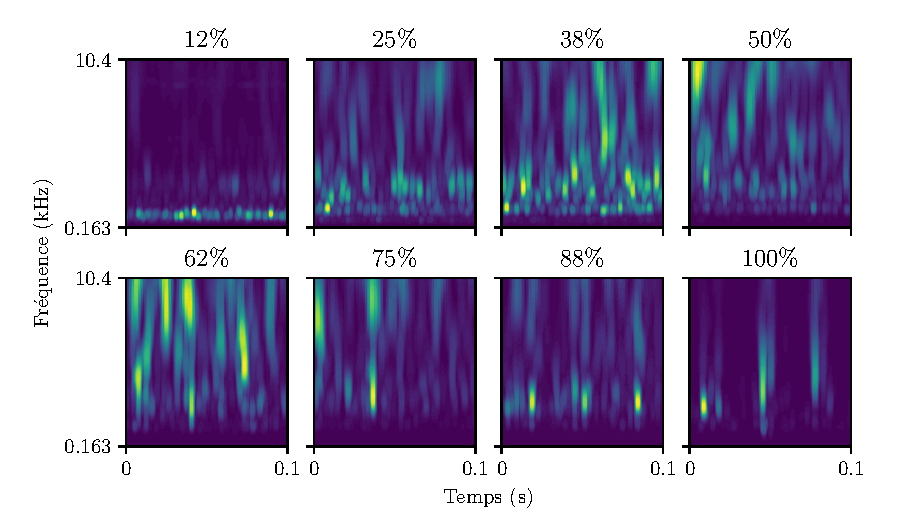
\includegraphics[]{figures/femtocwt_scaleograms_h_fr.pdf}
	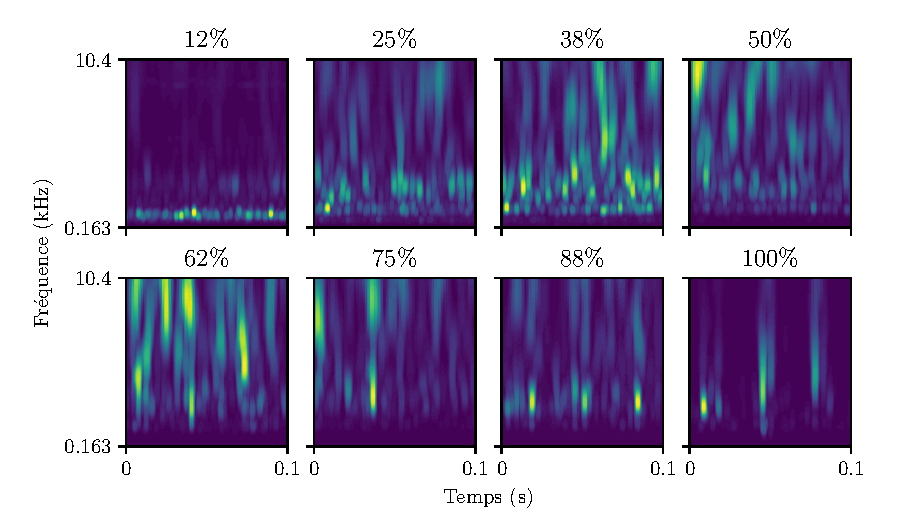
\includegraphics[]{figures/femtocwt_scaleograms_h_fr.png}
	\caption{Scalogrammes des différentes phases de la vie du roulement1\_1 (vibrations horizontales)}%
	\label{fig:bearings_fault_progress_scaleograms_h}
\end{figure}

\begin{figure}[h]
	\centering
	%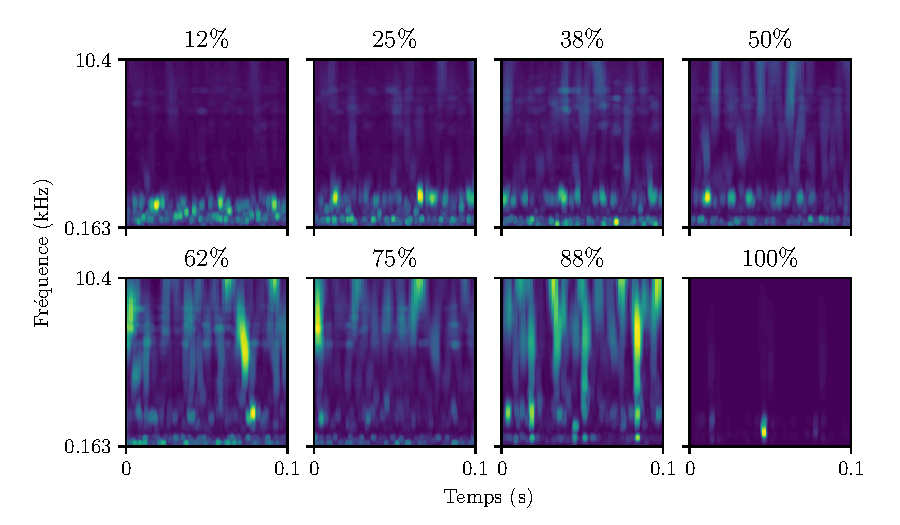
\includegraphics[]{figures/femtocwt_scaleograms_v_fr.pdf}
	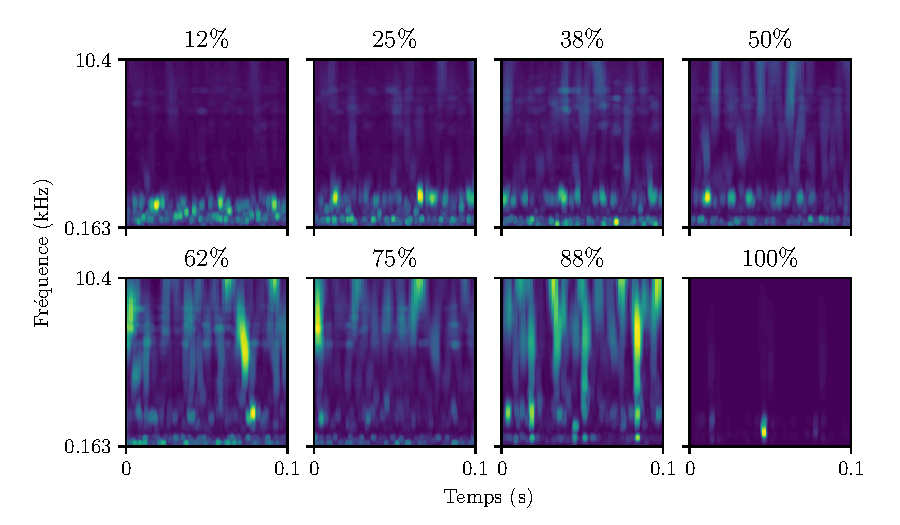
\includegraphics[]{figures/femtocwt_scaleograms_v_fr.png}
	\caption{Scalogrammes des différentes phases de la vie du roulement1\_1 (vibrations verticales)}%
	\label{fig:bearings_fault_progress_scaleograms_v}
\end{figure}

Les scalogrammes peuvent fournir des informations importantes sur l'état de santé du roulement, mais les différents roulements peuvent avoir des profils de dégradation différents. C'est pourquoi une base de données de scalogrammes est construite à partir des données de vibrations. Les 80 premiers enregistrements de vibrations de chaque roulement sont considérés comme représentant un roulement en bonne santé, tandis que les 80 derniers enregistrements de vibrations sont considérés comme défectueux. Ceci est considéré comme une tâche de classification binaire, où un réseau de neurones convolutifs sera utilisé pour extraire automatiquement les caractéristiques des bases de données des scaleogrammes (données de vibrations horizontales et verticales) et classifier l'état de santé du roulement. Pour éviter la complexité et le coût de l'entraînement d'un grand modèle, les scaleogrammes sont redimensionnés à une forme de (128$\times$128), de sorte que l'entrée du réseau est de forme (2$\times$128$\times$128) où les deux canaux correspondent aux scaleogrammes de vibrations horizontales et verticales. Ces données représentent les roulements de la première condition de fonctionnement (du Roulement1\_1 au Roulement1\_7).

\subsection{Détection de la défaillance des roulements à l'aide de réseaux de neurones convolutifs}%
\label{sub:detecting_bearings_failure_using_convolutional_neural_networks}

\subsubsection{Architecture de réseau}%
\label{subsub:network_architecture}
Pour cette tâche, un réseau de neurones convolutionnel (\acrshort{cnn}) avec 3 couches convolutionnelles, 3 couches de maxpooling et 3 couches entièrement connectées est utilisé. L'architecture complète du réseau avec le nombre de paramètres dans le réseau est représentée dans le tableau \ref{table:scaleograms-classifier-architecture}.

\begin{table}[ht]
    \centering
    \begin{tabu}{lll}
\tabucline[1.5pt]{-}
		\textbf{Couche (type)}   & \textbf{Forme de la sortie} &   \textbf{Param \#} \\
\tabucline[1pt]{-}
Conv1 (Conv2D)		&	(None, 2, 128, 16)	&	18448\\
MaxPool1 (MaxPooling2D) &    (None, 1, 64, 16)		&	0\\
Conv2 (Conv2D)          &    (None, 1, 64, 32)         	&	4640\\
MaxPool2 (MaxPooling2D) &    (None, 1, 32, 64)         	&	0\\
Conv3 (Conv2D)          &    (None, 1, 32, 128)        	&	18496\\
MaxPool3 (MaxPooling2D) &    (None, 1, 16, 128)        	&	0\\
Flatten1 (Flatten)      &   (None, 2048)              	&	0\\
Dense1 (Dense)          &    (None, 1024)              	&	524800\\
Dropout1 (Dropout)	&	(None, 512)		&	0\\
Dense2 (Dense)          &    (None, 64)                	&	32832\\
Dropout2 (Dropout)	&	(None, 64)		&	0\\
Dense3 (Dense)          &    (None, 2)                 	&	66\\
\tabucline[1pt]{-}
Total params: 559,346 &				&	\\
Trainable params: 599,346				&	\\
Non-trainable params: 0&				&	\\
	\tabucline[1.5pt]{-}
    \end{tabu}
    \caption{Architecture du classificateur de l'état de santé de roulements}
    \label{table:scaleograms-classifier-architecture}
\end{table}

\subsubsection{Processus d'entraînement}%
\label{subsub:training_process}
La base de données générée contenait un total de 1120 échantillons, 716 échantillons ont été utilisés pour l'entraînement, 180 pour la validation et 224 pour le test. Le réseau a été entraîné pour 50 époques avec des lots de 64 échantillons. La figure \ref{fig:scaleogram-classifier-training} montre le processus d'entraînement.

\begin{figure}[H]
	\centering
	\includegraphics{figures/femtocwt_training_fr.pdf}
	\caption{Entraînement du classificateur de l'état de santé des roulements}%
	\label{fig:scaleogram-classifier-training}
\end{figure}

\subsubsection{Discussion des résultats}%
\label{subsub:results-discussion}
Le réseau a atteint une exactitude d'entraînement parfaite de 100 \% et une exactitude de validation et de test similaire d'environ 98 \%. Le tableau \ref{table:femto-cwt-results} montre la perte et l'exactitude des données sur l'entraînement, la validation et les tests. Le tableau \ref{table:femto-cwt-metrics} montre les indicateurs supplémentaires de précision, de rappel et de score F-1.

\begin{table}[H]
	\centering
	\begin{tabu}{lcc}
		\tabucline[1.5pt]{2-3}
		&			\textbf{Perte}	&	\textbf{Exactitude}	\\
	   \tabucline[1pt]{-}
		Ensemble d'entraînement &	0.0017	&	100.00\%		\\
		Ensemble de validation 	&	0.0528 	&	98.89\%			\\
		Ensemble de test	&	0.0527 	&	98.44\%			\\
   \tabucline[1.5pt]{-}
   \end{tabu}
   \caption{Résultats de l'entraînement du classificateur de l'état de santé de roulements}
   \label{table:femto-cwt-results}
\end{table}


\begin{table}[H]
    \centering
    \begin{tabu}{cccccc}

    \tabucline[1.5pt]{-}
    \textbf{Métrique} &  \textbf{Exactitude} &  \textbf{Précision} &  \textbf{Rappel} &  \textbf{F-1} &  \textbf{ROC AUC}  \\
    \hline
  \textbf{Valeur} & 98.44\% & 0.9896 & 0.9694 & 0.9794 & 0.8348 \\
	\tabucline[1.5pt]{-}
    \end{tabu}
    \caption{Indicateurs supplémentaires pour la performance du réseau}
    \label{table:femto-cwt-metrics}
\end{table}

La figure \ref{fig:bearings_health_state_classifier_roc} montre la courbe ROC du classificateur :

\begin{figure}[H]
	\centering
	\includegraphics[]{figures/femtocwt_roc_auc_fr.pdf}
	\caption{Courbe ROC du classificateur de l'état de santé des roulements sur l'ensemble de test}%
	\label{fig:bearings_health_state_classifier_roc}
\end{figure}

\subsection{Le besoin de nouvelles caractéristiques de pronostic}%
\label{sub:the_need_for_appropriate_features}
L'entrée du modèle de pronostic est essentielle à la précision de ses prédictions \cite{coble2009} et puisque c'est le cas, une étape de sélection des caractéristiques doit être effectuée lors du développement du modèle, qui vise à sélectionner un ensemble de caractéristiques appropriées qui peuvent rendre la prédiction plus précise \cite{javed2012}. C'est pourquoi il est important d'utiliser des mesures concrètes qui peuvent quantifier la qualité des caractéristiques pronostiques sélectionnées et aider à les comparer directement et à sélectionner les plus appropriées.

\subsubsection{Trendabilité et monotonicité}%
\label{subsub:trendability_and_monotonicity}
Dans \cite{coble2009}, les auteurs ont proposé un ensemble de mesures qui peuvent être utilisées pour quantifier la qualité des caractéristiques de pronostic et comparer directement leur aptitude à être utilisées dans des modèles prédictifs, deux de ces mesures sont \textbf{monotonicité} et \textbf{trendabilité}. Selon leur définition, la monotonicité fait référence à la nature de la variable, qu'elle soit croissante ou décroissante, et elle a une valeur comprise entre 0 et 1, une variable qui est toujours croissante ou décroissante ayant une monotonicité de 1. La monotonicité est définie par l'équation \ref{equation:monotonicity} :

\begin{equation}
	M=\frac{\text{no. of }\frac{d}{dx} > 0}{n-1} - \frac{\text{no. of }\frac{d}{dx} < 0}{n-1}
\label{equation:monotonicity}
\end{equation}

La tendabilité, en revanche, a été définie comme le fait de savoir si une caractéristique donnée suit la même tendance (à la hausse ou à la baisse) dans une population de systèmes. Une caractéristique qui est toujours à la baisse ou à la hausse a une plus grande tendance qu'une autre qui ne suit pas une tendance spécifique dans différents cas. En conséquence, la tendance est définie par l'équation \ref{equation:trendability} :

\begin{equation}
	\begin{aligned}
		t_i&= \frac{\text{no. of }\frac{d}{dx}>0}{n-1}+\frac{\text{no of } \frac{d^2}{dx^2}>0}{n-2}\\
Trendability&=1-std(t_i)
	\end{aligned}
	\label{equation:trendability}
\end{equation}

\subsection{Caractéristiques trigonométriques et descripteurs cumulatifs}%
\label{sub:trigonometric_features}

Dans \cite{javed2013}, les auteurs ont proposé une nouvelle procédure d'extraction des caractéristiques des données de vibration basée sur une transformée en ondelettes discrètes (Section \ref{subsub:transformation_en_ondelettes_discretes}) et des fonctions trigonométriques. D'abord, le signal de vibration brut est décomposé en utilisant une transformée en ondelettes discrètes avec une ondelette db4 et un 4ème niveau de décomposition, puis les coefficients de décomposition sont mis à l'échelle en utilisant des fonctions trigonométriques (par exemple asinh, atan), enfin l'écart-type des coefficients mis à l'échelle est calculé pour obtenir la valeur finale. Selon les auteurs, ces fonctions sont moins sensibles au bruit et à la variabilité des signaux de vibration bruts.

Le tableau \ref{table:trigonometric-classic_features} montre la définition mathématique des différentes caractéristiques classiques et trigonométriques utilisées dans le littérature :


\begin{table}[ht]
    \centering
    \begin{tabu}{ll}
		\tabucline[1.5pt]{-}
		\textbf{Trigonometric features}   & \textbf{Formula} \\
		\tabucline[1pt]{-}
		Standard deviation of asinh &   $\sigma\left(log\left[x_j+\sqrt(x_j^2+1)\right]\right)$  \\
		Standard deviation of atan  &   $\sigma\left(\frac{i}{2}log\left(\frac{i+x_j}{i-x_j}\right)\right)$ \\
					    &  \\
		\textbf{Classic features} & \textbf{Formula}\\
		\tabucline[1pt]{-}
		Entropy & $E(x)=\sum_jE(x_j)$ \\
		Energy & $e=\sum_{j=0}^nx_j^2$\\
		Root mean square & $RMS=\sqrt{\frac{1}{n}(x_1^2+\ldots+x_n^2)}$\\
		Skewness &  $\frac{\sum_{j=1}^n(x_j-\bar{X})^3}{(n-1)\sigma^3}$\\
		Kurtosis &  $\frac{\sum_{j=1}^n(x_j-\bar{X})^4}{(n-1)\sigma^4}$\\
		Upper bound & $max(x)+\frac{1}{2}\frac{max(X)-min(X)}{n-1}$\\
	\tabucline[1.5pt]{-}
    \end{tabu}
    \caption{Caractéristiques trigonométriques et classiques de pronostic \cite{javed2013}}
    \label{table:trigonometric-classic_features}
\end{table}

La figure \ref{fig:trigonometric_features_bearing1_1} montre deux caractéristiques trigonométriques (asinh et atan) pour le palier 1\_1 à partir de la base de données FEMTO. Elles ont été filtrées à l'aide du filtre Savitsky--Golay pour réduire le bruit et la variabilité.

\begin{figure}[h]
	\centering
	\includegraphics[width=0.8\linewidth]{figures/trigonometric_features.pdf}
	\caption{Caractéristiques trigonométriques du roulement1\_1}%
	\label{fig:trigonometric_features_bearing1_1}
\end{figure}


Même si les caractéristiques trigonométriques sont moins sensibles au bruit que les caractéristiques classiques (par exemple: rms, skewness, kurtosis, etc.), ce n'est pas toujours le cas. ), ce n'est pas toujours le cas. Les auteurs ont également proposé l'utilisation de descripteurs cumulatifs (c'est-à-dire la somme cumulative) afin d'assurer la monotonicité des caractéristiques. La caractéristique cumulative associée à chaque caractéristique est calculée selon l'équation \ref{equation:cumulative_features} :

\begin{equation}
Cf_{nk} = \frac{\sum_{i=1}^n f_{ik}} {\sqrt{abs\left(\sum_{i=1}^nf_{ik}\right)}}
\label{equation:cumulative_features}
\end{equation}

Dans la figure \ref{fig:trig_classic_cumulative_features}, les caractéristiques classiques et trigonométriques cumulées sont comparées à leurs homologues non cumulées. Même avec une simple inspection visuelle, il est évident que l'utilisation de descripteurs cumulatifs améliore considérablement la qualité des caractéristiques de pronostic en réduisant le bruit et les fluctuations.

\begin{figure}[H]
	\centering
	\includegraphics[width=0.8\linewidth]{figures/trig_classic_cumulative_features.pdf}
	\caption{Caractéristiques cumulatives classiques et trigonométriques}%
	\label{fig:trig_classic_cumulative_features}
\end{figure}

Pour quantifier l'amélioration causée par l'utilisation de descripteurs cumulatifs sur les caractéristiques de pronostic, la monotonicité et la trendabilité de chaque caractéristique et de sa contrepartie cumulative sont calculées et résumées dans les tableaux \ref{table:trigonometric-classic-monotonicity} et \ref{table:trigonometric-classic-trendability} respectivement.

\begin{table}[ht]
\centering
\begin{tabu}{cc|cc}
\tabucline[1.5pt]{-}
Feature & Monotonicity & Cumulative Feature & Monotonicity \\
\hline
$\sigma(atan)$ & 0.486 & C-$\sigma(atan)$ & 1 \\
$\sigma(asinh)$ & 0.481 & C-$\sigma(asinh)$ & 1 \\
kurtosis & 0.059 & C-kurtosis & 0.998 \\
entropy & 0.035 & C-entropy & 1 \\
rms & 0.481 & C-rms & 1 \\
ubound & 0.287 & C-ubound & 1\\
\tabucline[1.5pt]{-}
\end{tabu}
\caption{Différence de monotonicité entre les caractéristiques trigonométriques et classiques et leurs descripteurs cumulés}
\label{table:trigonometric-classic-monotonicity}
\end{table}

\begin{table}[ht]
\centering
\begin{tabu}{cc|cc}
\tabucline[1.5pt]{-}
Feature & Trendability & Cumulative Feature & Trendability \\
\hline
$\sigma(atan)$ & 0.987 & C-$\sigma(atan)$ & 0.993 \\
$\sigma(asinh)$ & 0.989 & C-$\sigma(asinh)$ & 0.995 \\
kurtosis & 0.985 & C-kurtosis & 0.890 \\
entropy & 0.994 & C-entropy & 0.976 \\
rms & 0.988 & C-rms & 0.993 \\
ubound & 0.990 & C-ubound & 0.996\\
\tabucline[1.5pt]{-}
\end{tabu}
\caption{Différence de trendabilité entre les caractéristiques trigonométriques et classiques et leurs descripteurs cumulés}
\label{table:trigonometric-classic-trendability}
\end{table}

Il est très évident que la monotonicité des caractéristiques a augmenté de manière significative pour les caractéristiques cumulatives par rapport aux caractéristiques non cumulatives. Mais pour la trendabilité, la différence était moins importante. La figure \ref{fig:features_fitness} montre la monotonicité (axe x) et la trendabilité (axe y) des deux types de caractéristiques :

\begin{figure}[H]
	\centering
	\includegraphics{figures/featuresfitness_fr.pdf}
	\caption{Features fitness}%
	\label{fig:features_fitness}
\end{figure}

\section{Application aux équipements des chantiers pétroliers}%
\label{sec:application_to_oilfield_equipment}

\subsection{Top Drive}%
\label{sub:top_drive}

Dans les platesformes de forage pétrolier, le Top Drive est un dispositif qui sert à faire tourner le train de sonde et à remplacer la table de rotation classique et la tige carrée. Le principal avantage de Top Drive par rapport aux solutions conventionnelles est la possibilité de forer en utilisant trois joints de tiges au lieu d'un seul, ce qui réduit considérablement le temps de forage. Top Drives aide également les foreurs à minimiser le coût et la fréquence des incidents liés aux tiges coincées \cite{slbtopdrive}.

Figure \ref{fig:figures/bentec_500_ht} montre le Top Drive Bentec 500-HT.

\begin{figure}[h]
	\centering
	\includegraphics[width=0.9\linewidth]{figures/bentec_500_ht.jpg}
	\caption{Top Drive Bentec 500-HT}%
	\label{fig:figures/bentec_500_ht}
\end{figure}

D'un point de vue technique, les Top Drives sont des systèmes beaucoup plus compliqués que les tables de rotation conventionnelles et les tiges carrées, ils ont donc besoin de programmes de maintenance plus rigoureux pour assurer leur disponibilité compte tenu de leur rôle majeur dans les opérations de forage. Chaque année, la technologie du pétrole et du gaz est poussée plus loin, pour forer dans des conditions plus difficiles et pour forer des puits de pétrole plus profonds et plus difficiles, ce qui impose des exigences plus strictes aux équipements utilisés : être capable de supporter des conditions plus difficiles tout en maximisant sa disponibilité, ce qui est d'une grande importance sur le terrain, par exemple le coût du temps d'arrêt des Top Drives peut atteindre 1m\$ par jour et causer des retards importants dans les opérations de forage \cite{skfbrochure}.

Dans \cite{Pournazari2016}, les auteurs ont rapporté un sondage réalisé dans l'industrie pour évaluer l'impression de différents groupes de personnes (opérateurs, entrepreneurs, constructeurs des appareils de forage...) sur l'utilisation de Top Drives. Le sondage a montré un niveau de satisfaction moyen de 60 \% pour tous les groupes interrogés, ce qui indique que les Top Drives ne répondent pas vraiment aux attentes de l'industrie. On leur a également demandé quelles étaient les caractéristiques qu'ils aimeraient voir dans Top Drives, les choses les plus souhaitées étant une réduction des temps d'arrêt et une meilleure capacité à détecter les pannes avant que le système ne tombe en panne. Cela signifie qu'une maintenance préventive et une approche pronostique plus fiables sont les améliorations les plus souhaitées de ces systèmes sur le terrain.

\subsection{Les composants de Top Drive}%
\label{sub:top_drive_components}

Les Top Drives sont constitués de nombreux sous-ensembles qui sont présentés dans la figure \ref{fig:topdrive-subassemblies}\footnote{Toutes les figures suivantes des composants Top Drive sont extraites du bulletin technique de Bentec pour les Top Drives TD-500-HT et TD-350-HT}.

\begin{figure}[H]
	\centering
	\includegraphics[width=\linewidth]{figures/topdrive_subassemblies.png}
	\caption{Sous-ensembles du Top Drive Bentec 500-HT}%
	\label{fig:topdrive-subassemblies}
\end{figure}

Le sous-ensemble Top Drive qui nous intéresse ici est l'unité de forage (Figure \ref{fig:topdrive-drillingunit}) qui est chargée de générer le mouvement de rotation et de le transférer au train de sonde. L'unité de forage est composée d'un cadre de protection, d'une unité hydraulique, d'une alimentation en boue, d'un ensemble de suspension et\textemdash  le plus important pour la discussion actuelle\textemdash  d'un entraînement.

\begin{figure}[H]
	\centering
	\includegraphics[width=.7\linewidth]{figures/topdrive_drillingunit.png}
	\caption{Unité de forage du Top Drive Bentec 500-HT}%
	\label{fig:topdrive-drillingunit}
\end{figure}

L'entraînement lui-même est composé de :

\begin{itemize}
	\item Engine cooling system
	\item Brake
	\item AC Motor
	\item Gearbox (Figure \ref{fig:topdrive-drillingunit-drive-components}(a))
	\item Mainshaft (Figure \ref{fig:topdrive-drillingunit-drive-components}b)
\end{itemize}

\begin{figure}[H]
	\centering
	\begin{subfigure}[t]{0.4\textwidth}
         \centering
	 \includegraphics[width=.7\textwidth]{figures/topdrive_drillingunit_drive_gearbox.png}
	 \label{fig:topdrive-drillingunit-drive-gearbox}
	 \caption{Boite de vitesses de l'entraînement}
     \end{subfigure}%
     \begin{subfigure}[t]{0.4\textwidth}
         \centering
 \includegraphics[width=0.7\textwidth]{figures/topdrive_drillingunit_drive_mainshaft.png}
	 \label{fig:topdrive-drillingunit-drive-mainshaft}
	 \caption{Arbre principal de l'entraînement}
     \end{subfigure}
	\caption{Les composants principals de l'entraînement}%
	\label{fig:topdrive-drillingunit-drive-components}
\end{figure}

La boîte de vitesses comporte deux étages avec un rapport de transmission de 14:1. La vitesse du moteur est réduite deux fois puis transférée à l'engrenage (1) de la boîte de vitesses. La transmission est située sur le palier de butée. La lubrification de la boîte d'engrenages est effectuée par une librification combinée par barbotage et pression (3). L'arbre principal (4) est alimenté par la transmission de la boîte de vitesses et se trouve dans la boîte de vitesses avec le palier de butée (2) et il est conduit par le palier inférieur (3). Un tuyau de lavage (1) est connecté pour exécuter le fluide de forage. L'arbre principal contient également le collier de charge (5) qui porte l'adaptateur de liaison à la tige de forage.

La figure \ref{fig:skf_tapered_roller_thrust_bearing} montre un exemple de palier conique habituellement utilisé dans les entraînements Top Drives. La figure \ref{fig:skf_topdrive} montre le palier dans un entraînement Top Drive.

\begin{figure}[H]
	\centering
	\includegraphics[width=0.6\linewidth]{figures/skf_tapered_roller_thrust_bearing.png}
	\caption{Palier de butée à rouleaux coniques SKF \cite{skf_tapered_roller_thurst_bearing}}%
	\label{fig:skf_tapered_roller_thrust_bearing}
\end{figure}

\begin{figure}[H]
	\centering
	\includegraphics[width=0.7\linewidth]{figures/skf_topdrive.png}
	\caption{Position des roulements dans le Top Drive \cite{skf_bearing}}%
	\label{fig:skf_topdrive}
\end{figure}

\subsection{Proposed approach for Top Drive monitoring using neural networks}%
\label{sub:proposed_approach_for_top_drive_monitoring_using_neural_networks}

Les Top Drives sont déjà équipés de nombreux capteurs pour surveiller leur état comme des capteurs de température, de pression et de débit, mais l'information que ces capteurs ne sont utilisés que de manière simplifiée par les opérateurs \cite{Pournazari2016}. Afin d'améliorer les programmes de maintenance et d'adopter des approches de maintenance préventive et de pronostic, une approche plus sophistiquée et méthodologique du traitement des données fournies par ces capteurs doit être utilisée, ainsi que l'introduction de nouveaux capteurs de vibrations qui sont les principaux capteurs de surveillance utilisés pour les roulements et les engrenages, les éléments présents dans le Top Drive et qui travaillent sous des charges élevées et variables.

La figure \ref{fig:topdrive-drive-sensors} est une représentation schématique simplifiée des procédures proposées pour employer des capteurs supplémentaires (points rouges) pour les vibrations dans l'entraînement afin de surveiller différents éléments comme les engrenages et les roulements. Il faudrait installer suffisamment de capteurs pour capter les vibrations dans les trois axes : les vibrations verticales, horizontales et axiales. Lorsque le Top Drive est en service, les données recueillies par ces capteurs peuvent être utilisées pour développer une architecture de réseau de neurones afin de détecter la dégradation des roulements (Section \ref{sec:etude_de_cas_pronostique_des_roulements}) ou---si suffisamment de données historiques sont disponibles---classer les différents modèles de dégradation (Section \ref{sec:etude_de_cas_diagnostique_des_roulements}). La détection correcte des dégradations ou même la classification des modèles de dégradation peut être utilisée pour planifier et préparer les actions de maintenance appropriées et les exécuter en temps voulu avant qu'une dégradation grave ne se produise, ce qui peut entraîner un temps improductif important et des coûts de maintenance corrective élevés.


\begin{figure}[H]
	\centering
	\begin{tikzpicture}
	\tikzstyle{gear} = [rectangle,  draw, align=center, darkgray, fill=gray, text=white]
	\tikzstyle{bearing} = [rectangle, draw, align=center]
	\tikzstyle{shaft} = [rectangle, draw, minimum width = 1em, fill=darkgray, darkgray]
	\tikzstyle{sensor}  = [circle, fill,red, minimum size=5,inner sep=0]
	\draw[black!20!white, thick, fill=black!5!white ] (0,0) rectangle (18em,-8em);
	\node[] at (2.5em,-1em) {Gearbox};

	\node[gear, minimum width=8em, minimum height=2em] at (7em,-4em) (gear) {Gear};
	\node[gear, minimum width=4em, minimum height=2em, right = 0em  of gear] (pinion) {Pinion};

	\node[bearing, minimum width=7em, minimum height=2em, below = 0em of gear] (thrustbearing) {\footnotesize Thrust bearing};

	\node[shaft, minimum height=4em, above = 0em of pinion] (shaft) {};
	\node[draw, thick, minimum width=3em, rounded corners, radius=3,minimum height=5em, above = 0em of shaft] {AC Motor};

	\node[shaft, minimum height=3em, below = 0em of thrustbearing] {};

	\node[sensor, below = 0em of thrustbearing] {};
	\node[sensor, left = 0em of thrustbearing] {};
	\node[sensor, above = 0em of gear] {};
	\node[sensor, left = 0em of gear] {};
	
\end{tikzpicture}	

	\caption{Approche proposée pour la surveillance du Top Drive à l'aide de réseaux de neurones}%
	\label{fig:topdrive-drive-sensors}
\end{figure}

\section{Conclusion}
Ce chapitre présente deux approches différentes pour le diagnostic et le pronostic des roulements à partir des données de vibrations. Les réseaux de neurones présentés ont permis d'obtenir une très grande exactitude de test. Ensuite, une méthodologie a été présentée pour intégrer ces modèles neuronaux dans les équipements critiques des champs pétrolifères (c'est-à-dire les entraînements Top Drives), ce qui peut avoir un grand impact sur les programmes de maintenance traditionnels existants et contribuer à réduire les temps improductifs et les coûts élevés résultant de la panne de ces équipements importants.
